\documentclass[12pt]{article}
\usepackage[utf8]{inputenc}
\usepackage[T1]{fontenc}
\usepackage[spanish,es-lcroman]{babel}
\usepackage{amsmath}
\usepackage{amsthm}
\usepackage{bm}
\usepackage{amsfonts}
\usepackage{amssymb}
\usepackage{physics}
\usepackage{tikz}
\usepackage{float}
\usepackage{calc}
\usepackage[autostyle,spanish=mexican]{csquotes}
\usepackage[per-mode=symbol]{siunitx}
\usepackage{textcomp, gensymb}
\usepackage{multicol}
\usepackage{enumitem}
\usepackage{graphicx}
\usepackage{hyperref}
\usepackage{bookmark}
\usepackage{setspace}
\usepackage[left=2.00cm, right=2.00cm, top=2.00cm, 
     bottom=2.00cm]{geometry}
% \usepackage{Estilos/ColoresLatex}
\usepackage{makecell}
% \usepackage{subcaption}
\usepackage[skip=10pt, indent=30pt]{parskip}
% \usepackage{scalerel}
\usepackage{scalerel}[2016-12-29]
% \usepackage{biblatex}
\usepackage{cancel}
\usepackage{caption}
\usepackage{capt-of}
\usepackage[outdir=./Imagenes/]{epstopdf}

\graphicspath{{Imagenes/}}
\DeclareGraphicsExtensions{.png,.jpg,.eps}

\definecolor{ao}{rgb}{0.0, 0.0, 1.0}

\hypersetup{
    colorlinks=true,
    linkcolor=ao,
    filecolor=magenta,      
    urlcolor=ao,
}

\newcommand{\ptilde}[1]{\ensuremath{{#1}^{\prime}}}
\newcommand{\stilde}[1]{\ensuremath{{#1}^{\prime \prime}}}
\newcommand{\ttilde}[1]{\ensuremath{{#1}^{\prime \prime \prime}}}
\newcommand{\ntilde}[2]{\ensuremath{{#1}^{(#2)}}}
\newcommand{\pderivada}[1]{\ensuremath{{#1}^{\prime}}}
\newcommand{\sderivada}[1]{\ensuremath{{#1}^{\prime \prime}}}
\newcommand{\tderivada}[1]{\ensuremath{{#1}^{\prime \prime \prime}}}
\newcommand{\nderivada}[2]{\ensuremath{{#1}^{(#2)}}}

\def\stretchint#1{\vcenter{\hbox{\stretchto[440]{\displaystyle\int}{#1}}}}
\def\scaleint#1{\vcenter{\hbox{\scaleto[3ex]{\displaystyle\int}{#1}}}}
\def\scaleiint#1{\vcenter{\hbox{\scaleto[6ex]{\displaystyle\iint}{#1}}}}
\def\scaleiiint#1{\vcenter{\hbox{\scaleto[6ex]{\displaystyle\iiint}{#1}}}}
\def\scaleoint#1{\vcenter{\hbox{\scaleto[3ex]{\displaystyle\oint}{#1}}}}
\def\bs{\mkern-12mu}

% \newcommand{\textbf}[2]{\textbf{\textcolor{#1}{#2}}}
\sisetup{per-mode=symbol}
\decimalpoint
\sisetup{bracket-numbers = false}
\newlength{\depthofsumsign}
\setlength{\depthofsumsign}{\depthof{$\sum$}}
\newcommand{\nsum}[1][1.4]{% only for \displaystyle
    \mathop{%
        \raisebox
            {-#1\depthofsumsign+1\depthofsumsign}
            {\scalebox
                {#1}
                {$\displaystyle\sum$}%
            }
    }
}

\AtBeginDocument{\RenewCommandCopy\qty\SI}
\ExplSyntaxOn
\msg_redirect_name:nnn { siunitx } { physics-pkg } { none }
\ExplSyntaxOff

\numberwithin{equation}{section}

\linespread{1.25}

\renewcommand{\labelenumii}{\theenumii}
\renewcommand{\theenumii}{\theenumi.\arabic{enumii}.}

\emergencystretch=1em

\title{Función delta de Dirac}
\author{M. en C. Gustavo Contreras Mayén}
\date{ }

\begin{document}
\maketitle
\fontsize{14}{14}\selectfont
\spanishdecimal{.}
\tableofcontents
\newpage

\section{La delta de Dirac.}
\subsection{Impulsos en la física.}

En física a menudo nos encontramos con fenómenos donde se involucra el concepto de un pulso de duración \textbf{infinitamente corto}. Por ejemplo, en el curso de Mecánica Clásica se revisa el concepto de una magnitud física llamada \textbf{impulso}, la cual se introduce cuando se cambia el estado de movimiento de un cuerpo al aplicarle un \textbf{golpe repentino}. El impulso se denota comúnmente con la letra $I$.
\par
Tomemos como ejemplo del fútbol, con un penalty,  en este caso tenemos inicialmente al balón en reposo, la intención es meter la pelota en la portería contraria. Después de patear el balón, éste adquiere un momento que es igual al impulso asociado a la patada misma.
\par
Analíticamente esta afirmación se escribe como:
\begin{align*}
m \: v = I = \scaleint{6ex}_{t_{0}}^{t_{0} + \tau} F (t) \dd{t}
\end{align*}
donde $F (t)$ es la fuerza y $\tau$ la duración del impacto sobre la pelota (técnicamente de la acción de la fuerza sobre el balón). El término \textbf{repentino} implica que $\tau$ se considera infinitamente pequeño y por tanto, que el cambio en el momento ocurre instantáneamente.
\par
Sin embargo, dado que el cambio en el momento es un número finito, se sigue que la magnitud de la fuerza $F (t)$ debió haber sido infinita durante el golpe al balón y cero en cualquier otro momento. Este tipo de descripciones no se puede formular apropiadamente con los conceptos matemáticos que conocemos, más aún, la descripción tampoco es rigurosa desde un punto de vista físico.
\begin{figure}[H]
    \centering
    \includegraphics[scale=1]{Imagenes/delta_Dirac_01.eps}
    \caption{Representación del pico para la función.}
    \label{fig:delta_Dirac_01}
\end{figure}
En realidad, la gráfica de la fuerza es una curva muy \textbf{picuda}:
\begin{enumerate}
\item Es muy estrecha y muy alta, como se aprecia en la figura (\ref{fig:delta_Dirac_01})
\item Satisface la propiedad que el área bajo la curva es igual a $I$.
\end{enumerate}
En la gran mayoría de los problemas físicos, la forma exacta de la gráfica no se conoce,  sin embargo, en lo correspondiente a los efectos físicos observables asociados con tal función, usualmente esta falta de información no importa. Lo que tiene significado es la integral de la fuerza, esto es, el valor del impulso:
\begin{align*}
I = \scaleint{6ex}_{t_{0}}^{t_{0} + \tau } F (t) \dd{t}
\end{align*}
Las funciones puntiagudas son comunes en cualquier área de la física,  por ejemplo: una fuerza concentrada sobre una barra, es una distribución puntiaguda de la carga, ver la figura (\ref{fig:figura_delta_Dirac_02}). 
\begin{figure}[H]
    \centering
    \includegraphics[scale=1.3]{Imagenes/delta_Dirac_02a.eps}
    \caption{Distribución de carga ideal.}
    \label{fig:figura_delta_Dirac_02}
\end{figure}
\begin{figure}[H]
    \centering
    \includegraphics[scale=0.85]{Imagenes/delta_Dirac_02b.eps}
    \caption{Distribución de carga real.}
    \label{fig:figura_delta_Dirac_05}
\end{figure}

En los circuitos eléctricos, las corrientes \textbf{puntiaguadas} de una duración extremadamente corta, se presentan cuando se conecta el interruptor. Como en el caso de la redistribución de carga entre dos condensadores, como se ve en la figura (\ref{fig:figura_delta_Dirac_03}).
\begin{figure}[H]
    \centering
    \includegraphics[scale=1.25]{Imagenes/delta_Dirac_03.eps}
    \caption{Circuito eléctrico antes de cerrar el interruptor.}
    \label{fig:figura_delta_Dirac_03}
\end{figure}


\section{Dos definiciones de \texorpdfstring{$\delta (t)$}{d(t)}.}
\subsection{Dos enfoques.}

Hay dos formas comunes de definir la función $\delta$ de Dirac. El enfoque más riguroso, desde la teoría de funciones generalizadas, lo define por su comportamiento dentro de las operaciones integrales. De hecho, nunca se supone que la función $\delta$ exista fuera de una integral.
\par
En general, en ciencia e ingeniería se un poco más laxos y usan una segunda definición. A menudo definen la función $\delta$ como el límite de una secuencia infinita de funciones continuas.

\subsection{Como límite de una secuencia.}

La función $\delta$ puede verse como el límite de una secuencia de funciones, es decir:
\begin{align}
\delta(t) = \lim_{n \to \infty} \delta_{n} (t)
\label{eq:ecuacion_05_10}
\end{align}
donde $\delta_{n}(t)$ es finito para todos los valores de $t$.
\par
Hay muchas secuencias de funciones que se acercan a la función $\delta$ de Dirac de esta manera. La más simple es la secuencia de función cuadrada definida por:
\begin{align}
\delta_{n} (t) = \begin{cases}
n & -\dfrac{1}{2 \, n} < t < \dfrac{1}{2 \, n} \\
0 & \mbox{en cualquier otro punto}
\end{cases}
\label{eq:ecuacion_05_11}
\end{align}
como se muestra en la figura (\ref{fig:figura_05_06}).
\begin{figure}[H]
    \centering
    \includegraphics[scale=1]{Imagenes/plot_secuencia_delta_02.eps}
    \caption{Primeras tres funciones de la secuencia.}
    \label{fig:figura_05_06}
\end{figure}
Es claro que para cualquier valor de $n$:
\begin{align}
\scaleint{6ex}_{\bs -\infty}^{\infty} \delta_{n} (t) \dd{t} = 1
\label{eq:ecuacion_05_12}
\end{align}
en el límite cuando $n \to \infty$, $\delta_{n}(t) = 0$ para todo valor de $t$, excepto $t = 0$. 
\par
Hay otras tres secuencias de funciones comunes que se acercan a la función $\delta$ de Dirac: las secuencias de resonancia, gaussiana y sinc al cuadrado, se muestran en las siguientes figuras (\ref{fig:figura_05_07}) a (\ref{fig:figura_05_09}). Se describen matemáticamente mediante:
\begin{align}
\begin{aligned}
\mbox{Resonancia:} \hspace{1cm} \delta_{n}(t) &= \dfrac{n/\pi}{1 + n^{2} \, t^{2}} \\[1em]
\mbox{Gaussiana:} \hspace{1cm} \delta_{n}(t) &= \dfrac{n}{\sqrt{\pi}} \, e^{-n^{2} t^{2}} \\[1em]
\mbox{Sinc cuadrada:} \hspace{1cm} \delta_{n}(t) &= \dfrac{\sin^{2} n \, t}{n \, \pi \, t^{2}} 
\end{aligned}
\label{eq:ecuacion_05_13}
\end{align}

\newpage

Secuencia de resonancia.
\begin{figure}[H]
    \centering
    \includegraphics[scale=1]{Imagenes/secuencia_Delta_05.eps}
    \caption{Gráfica de la secuencia delta para la función resonancia.}
    \label{fig:figura_05_07}
\end{figure}
Cada una de esas funciones tiene un área unitaria para cualquier valor de $n$, y es fácil calcularla cuando en el límite $n \to \infty$, $\delta_{n} (t) = 0$ para todo $t \neq 0$.

Secuencia Gaussiana.
\begin{figure}[H]
    \centering
    \includegraphics[scale=1]{Imagenes/secuencia_Delta_06.eps}
    \caption{Gráfica de la secuencia delta para la función Gaussiana.}
    \label{fig:figura_05_08}
\end{figure}

\newpage

Secuencia sinc al cuadrado.
\begin{figure}[H]
    \centering
    \includegraphics[scale=1]{Imagenes/secuencia_Delta_07.eps}
    \caption{Gráfica de la secuencia delta para la función sinc al cuadrado.}
    \label{fig:figura_05_09}
\end{figure}

\subsection{Por operaciones integrales.}

En matemáticas, la función $\delta$ se define por cómo se comporta dentro de una integral. Cualquier función que se comporte como $\delta (t)$ en la siguiente ecuación es por definición una función $\delta$:
\begin{align}
\scaleint{6ex}_{\bs t_{-}}^{t_{+}} f (t) \, \delta(t - t_{0}) \dd{t} = \begin{cases}
f (t_{0}) & t_{-} < t_{0}  < t_{+} \\
0 & \mbox{en cualquier otro punto}
\end{cases}
\label{eq:ecuacion_05_14}
\end{align}
donde $t_{-} < t_{+}$ y $f (t)$ es cualquier función continua de buen comportamiento.

% \section{Distribuciones.}
% Las ideas que nos permitieron desarrollar el concepto de la delta de Dirac previamente, se pueden sistematizar en lo que se conoce como \emph{la teoría de distribuciones o funciones generalizadas}.
% \par
% Las funciones generalizadas fueron introducidas en 1935 por el matemático ruso, Sergei Lvóvich Sóbolev (1908 - 1989). De manera independientemente a finales de la década de 1940, el matemático francés, Laurent Schwartz (1915 - 2002) formalizó la teoría de distribuciones, lo que le valió la Medalla Fields en 1950 (que no recibió durante la entrega ya que se le negó la visa para ingresar a los Estados Unidos.)
% \par
% Como el nombre lo sugiere, la teoría tiene como objetivo  \emph{extender la definición de una función}, de manera tal que conceptos como el de la delta de Dirac $\delta (x)$ cuenten con una base matemática firme. En particular la teoría permite extender el concepto de derivada a todas las funciones localmente integrables y a entes aún más generales. Existen varias formas de presentar la teoría de distribuciones, se dará una breve introducción utilizando las integrales de secuencias de funciones del tipo
% \begin{equation}
% \int f_{n}(x) \: g(x) \dd{x} \hspace{1cm} n = 1, 2, 3 , \ldots
% \label{eq:ecuacion_1_99}
% \end{equation}
% Para ello es necesario introducir tres conceptos:
% \begin{enumerate}
% \item El concepto de función de prueba.
% \item El concepto de función admisible.
% \item El concepto de convergencia débil.
% \end{enumerate}
% Hemos visto que una secuencia de funciones $f_{n}(x)$ tal como la secuencia delta de funciones, definida en \ref{secuencias_delta}, nos lleva al concepto matemático de \enquote{función} delta, si la secuencia de integrales converge para funciones apropiadas $g(x)$. Pero ¿Qué quiere decir que sean apropiadas? En la sección anterior vimos que si queremos definir conceptos tales como las derivadas de la función delta, entonces las funciones $g(x)$ deben ser diferenciables. Para definir las derivadas también hemos visto que al integrar por partes, para que las derivadas totales no contribuyan, es necesario que la función $g(x)$ tenga un comportamiento apropiado en infinito. Definimos entonces las funciones $g(x)$ como
% \begin{defi}
% Funciones de prueba.
% Decimos que las función $g(x)$ en la ec. (\ref{eq:ecuacion_1_99}), es de prueba, si es infinitamente diferenciable (clase $C^{\infty}$) y es idénticamente cero fuera de algún intervalo $(a, b)$ (en general este intervalo es diferente para funciones $g(x)$ diferentes).
% \end{defi}
% El nombre de funciones de prueba es adecuado, dado que por ejemplo, la propiedad de filtro de las secuencias delta, se prueba sobre estas funciones. Habiendo definido las funciones de prueba, podemos ahora definir las funciones admisibles (de las cuales seleccionaremos las funciones $f_{n}(x)$ y la convergencia débil.
% \begin{defi}
% Funciones admisibles.

% Decimos que las funciones $f_{n}(x)$ en la ec. (\ref{eq:ecuacion_1_99}) son admisibles, si son infinitamente diferenciables. Su comportamiento en infinito puede ser arbitrario.
% \end{defi}
% \begin{defi}
% Convergencia débil.

% Consideremos una secuencia de funciones admisibles $f_{n}(x)$ con \\ $n = 1, 2, 3, \ldots$
% Decimos que esta secuencia es débilmente convergente si el límite
% \begin{equation}
% \lim_{n \to \infty} \scaleint{6ex}_{\bs -\infty}^{\infty} f_{n}(x) \:  g(x) \, \dd{x}
% \label{eq:ecuacion_1_100}
% \end{equation}
% existe para todas las funciones de prueba $g(x)$.
% \end{defi}
% Una secuencia débilmente convergente puede o no puede converger en alguno de los sentidos de convergencia usual, como convergencia puntual.
% \par
% Podemos presentar ahora una definición rigurosa de una distribución de la siguiente manera:
% \begin{defi}
% Distribuciones.

% Una distribución $\varphi (x)$ es un concepto matemático asociado con una secuencia débilmente convergente de funciones admisibles para la cual la integral simbólica
% \begin{equation}
% \scaleint{6ex}_{\bs -\infty}^{\infty} \phi (x) \:  g(x) \, \dd{x}
% \label{eq:ecuacion_1_101}
% \end{equation}
% tiene un significado preciso, por medio de la prescripción
% \begin{equation}
% \scaleint{6ex}_{\bs -\infty}^{\infty} \phi (x) \: g(x) \, dx = \lim_{n \to \infty} f_{n}(x) \: g(x) \, \dd{x}
% \label{eq:ecuacion_1_102}
% \end{equation}
% \end{defi}

\section{La delta de Dirac.}
\subsection{Definición informal de la delta de Dirac.}


¿Entonces qué es la delta de Dirac? Informalmente la delta de Dirac es una \enquote{función} que representa un pico infinitamente agudo expresado simbólicamente por:
\begin{align}
\delta (x) = \begin{cases}
0 & x \neq 0 \\
\infty & x = 0
\end{cases}
\label{eq:ecuacion_delta_01}
\end{align}
Pero tal que la integral de $\delta (x)$ está normalizada a la unidad:
\begin{equation}
\scaleint{6ex}_{\bs -\infty}^{\infty} \delta (x) \: \dd{x} = 1 
\label{eq:ecuacion_delta_02}
\end{equation}


\section{Propiedades de la delta de Dirac.}
\subsection{Conjunto de propiedades.}

Se presentarán una serie de propiedades de la delta de Dirac, que tomaremos como se indica, ya que nos serán de utilidad en varios momentos del curso de MAF.

\subsection{Propiedad de filtro.}

La delta de Dirac satisface la siguiente propiedad:
\begin{equation}
\scaleint{6ex}_{\bs -\infty}^{\infty} \delta (x) \: f (x) \: \dd{x} = f (0)
\label{eq:ecuacion_delta_03}
\end{equation}
donde $f(x)$ es una función continua.
\par
Esta integral puede ser \enquote{evaluada} utilizando siguiente argumento:  dado que $\delta (x) = 0$
para $x \neq 0$, podemos cambiar los límites de integración en la ecuación (\ref{eq:ecuacion_delta_03}) a $- \epsilon$ y $+ \epsilon$, donde $\epsilon$ es un número positivo infinitesimal. Más aún, dado que $f (x)$ es continua en $x = 0$, sus valores dentro del intervalo $( - \epsilon, + \epsilon)$ no diferirán mucho de $f(0)$. Y podemos hacer la siguiente aproximación:
\begin{align*}
&\scaleint{6ex}_{\bs -\infty}^{\infty} \delta (x) \: f (x) \: \dd{x} = \scaleint{6ex}_{\bs -\epsilon}^{\epsilon} \delta (x) \: f (x) \: \dd{x} \approx f(0) \scaleint{6ex}_{\bs -\infty}^{\infty} \delta (x) \: \dd{x}
\end{align*}
Esta aproximación mejora cuando $\epsilon \to 0$. Pero:
\begin{align*}
\scaleint{6ex}_{\bs -\epsilon}^{+\epsilon} \delta (x) \: \dd{x} = 1
\end{align*}
para todos los valores de $\epsilon$, por que $\delta (x) = 0$ para $x \neq 0$ y $\delta (x)$ está normalizada. Así en el límite $\epsilon \to 0$, se tiene que:
\begin{align*}
\scaleint{6ex}_{\bs -\infty}^{\infty} \delta (x) \: f (x) \: \dd{x} = f(0)
\end{align*}
\textbf{Nota: } Los límites $-\infty$ y $+\infty$ se pueden reemplazar por cualesquiera números $a$ y $b$, tales que $a < 0 < b$.
\par
Propiedad de filtro: La $\delta (x)$ actúa como un filtro, seleccionando de todos los posibles valores de $f (x)$ su valor en el punto $x = 0$.

\subsection{Filtro de las derivadas.}

Se presenta la propiedad para las derivadas de orden superior de $\delta (x)$:
\begin{align*}
\scaleint{6ex}_{\bs -\infty}^{+\infty} \dv[m]{\delta (x)}{x} \: f (x) \dd{x} =  (-1)^{m} \: \dv[m]{f (0)}{x}
\end{align*}
Es necesario enfatizar que la expresión anterior tiene significado sólo cuando asumimos directamente que las funciones involucradas son $m$ veces diferenciables y además, las integrales:
\begin{align*}
\scaleint{6ex}_{\bs -\infty}^{+\infty} \dv[k]{\phi_{n}(x)}{x} \: f (x) \dd{x}
\end{align*}
convergen para todo valor de $n$ y para todo valor de $k$ de $0$ a $m$.

\subsection{Producto por una función.}

Para el producto de la delta de Dirac con una función se tiene que:
\begin{align*}
x \: \delta(x) &= 0 \\[0.5em] 
f (x) \: \delta(x - a) &= f (a) \: \delta (x - a)
\end{align*}

\subsection{Paridad de la delta de Dirac y su derivada.}

La delta de Dirac es una función par:
\begin{align*}
\delta (-x) &= \delta (x) \\[0.5em] 
\pderivada{\delta} (-x) &= - \pderivada{\delta} (x)
\end{align*}

\subsection{Propiedad de escalamiento.}

Si se aplica una escala $a \neq 0$ a la variable dentro de la $\delta (x)$, el valor de la función cambia proporcionalmente al inverso del valor absoluto de esa escala:
\begin{align*}
\delta(a \, x) &= \dfrac{1}{\abs{a}} \: \delta (x), \hspace{1cm} a \neq 0
\end{align*}

\subsection{Más propiedades.}

\begin{align*}
&\delta (x^{2} - a^{2}) = \dfrac{1}{2 \, a} \bigg[ \delta (x + a) + \delta (x - a) \bigg] \hspace{1cm} a > 0 \\[1em]
&\delta (x - \pderivada{x}) = 0 \hspace{1cm} x \neq \pderivada{x} \\[1em]
&\scaleint{6ex}_{\bs a}^{b} \delta (x - \pderivada{x}) \dd{\pderivada{x}} = 1 \hspace{1cm} a < x < b \\[1em]
&\delta (x - \pderivada{x}) = \delta (\pderivada{x} - x) \\[1em]
&\scaleint{6ex}_{\bs -\infty}^{+\infty} f (\pderivada{x}) \delta (x - \pderivada{x}) \dd{\pderivada{x}} = f (x) \\[1em]
&\scaleint{6ex}_{\bs -\infty}^{+\infty} \delta (\sderivada{x} - \pderivada{x}) \, \delta (\pderivada{x} - x) \dd{\sderivada{x}} = \delta (\pderivada{x} - x) \\[1em]
&\delta ( f(x) ) = \nsum_{i=1}^{N} \dfrac{\delta (x - x_{i})}{\abs{\pderivada{f} (x)}}_{x=x_{i}}
\end{align*}

% \subsection{Secuencias delta.}\label{secuencias_delta}
% La afirmación de que la función $\delta (x)$ está dada por la expresión (\ref{eq:ecuacion_delta_01}) \textit{no es una afirmación apropiada y no se puede utilizar para definir una función}, mucho menos para una función integrable. Una posible definición alterna, podría ser el definir la función $\delta (x)$ como la función que satisface la propiedad de filtro (\ref{eq:ecuacion_delta_03})
% \begin{align*}
% \scaleint{6ex}_{\bs -\infty}^{+ \infty} \delta (x) \: f(x) \: \dd{x} = f(0)
% \end{align*}
% para toda función continua $f(x)$. Sin embargo es posible demostrar que no existe ninguna función con esa propiedad. Por lo que 
% \begin{center}
% \textit{¡¡la función delta no es una función en el sentido matemático usual!!}
% \end{center}
% ¿Qué se hace entonces?  ¿Dirac nos engañó con su propuesta? Lo que sucede es que existen secuencias de funciones de pico pronunciado, las cuales en el límite en que el pico es infinitamente delgado e infinitamente alto, satisfacen la propiedad de filtro.
% \par
% La siguiente puede ser una secuencia $\phi_{n} (x)$ con $n = 1, 2, 3, \ldots$, tal que
% \begin{align*}
% \lim_{n \to \infty} \scaleint{6ex}_{\bs -\infty}^{+ \infty} \phi_{n}(x) \: f(x) \dd{x} =  f(0)
% \end{align*}
% \begin{defi}
% Llamamos secuencias delta $\delta_{n} (x)$ a una secuencia de funciones de pico pronunciado, que satisfacen
% \begin{align*}
% \lim_{n \to \infty} \scaleint{6ex}_{\bs -\infty}^{+ \infty} \phi_{n} (x) \: f(x) \: \dd{x} =  f(0)
% \end{align*}
% \end{defi}
% \begin{ejemplo}
% La secuencia de funciones
% \begin{equation}
% \phi_{n} (x) = \begin{cases}
% 0 & x < - \dfrac{1}{2 \, n} \\
% n & - \dfrac{1}{2 \, n} < x < \dfrac{1}{2 \, n} \\
% 0 & 0 >  \dfrac{1}{2 \, n}
% \end{cases}
% \hspace{1cm} n = 1, 2, 3, \ldots
% \label{eq:ecuacion_delta_04}
% \end{equation}
% es una secuencia delta.
% \end{ejemplo}
% \begin{figure}[H]
% \centering
% \includestandalone{./Figuras/plot_secuencia_delta}
% \caption{Secuencia delta para valores de $n=1,2,\ldots,10$. El área debajo de la curva para cada $\phi_{n}$ siempre es $1$.}
% \label{fig:secuncia_delta_01}
% \end{figure}
% Para verificar esta afirmación consideremos la integral
% %Apuntes FETI página 46
% \begin{align*}
% \scaleint{6ex}_{\bs -\infty}^{\infty} \phi_{n} (x) \: f(x) \dd{x}
% \end{align*}
% para cualquier función continua arbitraria $f(x)$. De la expresión (\ref{eq:ecuacion_delta_04}) para la secuencia delta se tiene
% \begin{align*}
% \scaleint{6ex}_{\bs -\infty}^{+ \infty} \phi_{n} (x) \: f(x) \dd{x} = \scaleint{6ex}_{\bs -\frac{1}{2 \, n}}^{\frac{1}{2 \, n}} n \: f(x) \: \dd{x} = n \scaleint{6ex}_{\bs -\frac{1}{2 \, n}}^{\frac{1}{2 \, n}} f(x) \:  \dd{x}
% \end{align*}
% Utilizando el teorema del valor medio para integrales, podemos deducir que
% \begin{align*}
% n \scaleint{6ex}_{\bs -\frac{1}{2 \, n}}^{\frac{1}{2 \, n}} f(x) \dd{x} = n \: \dfrac{1}{n} f(\xi) = f(\xi), \hspace{1cm} - \dfrac{1}{2 \, n} \leq \xi \leq \dfrac{1}{2 \, n}
% \end{align*}
% En el límite cuando $n \to \infty$, $\xi \to 0$. De la continuidad de la función $f(x)$ se sigue que $f(\xi) \to f(0)$, obteniendo así el resultado
% \begin{align*}
% \lim_{n \to \infty} \scaleint{6ex}_{\bs -\infty}^{+ \infty} \: \phi_{n}(x) \: f(x) \: \dd{x} = f(0)
% \end{align*}
% lo que nos dice que la secuencia (\ref{eq:ecuacion_delta_04}) es una secuencia delta.
% \par
% Nótese que la secuencia delta (\ref{eq:ecuacion_delta_04}) no es derivable en el punto $x = 0$. Para muchos propósitos es deseable
% construir secuencias delta de funciones que sean continuas y diferenciables. Por ejemplo, en las figuras (\ref{fig:plot_secuencia_01}), (\ref{fig:plot_secuencia_02}) y (\ref{fig:plot_secuencia_03}) podemos apreciar algunas secuencias delta con estas características:

% \begin{figure}[H]
%     \centering
%     \includegraphics[scale=0.8]{Imagenes/secuencia_delta_01.eps}
%     \caption{Secuencia para $\phi_{n}$ con $n=1,2,3$}
%     \label{fig:plot_secuencia_01}
% \end{figure}


% \begin{figure}[H]
%     \centering
%     \includegraphics[scale=0.8]{Imagenes/secuencia_delta_02.eps}
%     \caption{Secuencia para $\phi_{n}$ con una función exponencial.}
%     \label{fig:plot_secuencia_02}
% \end{figure}

% \begin{figure}[H]
%     \centering
%     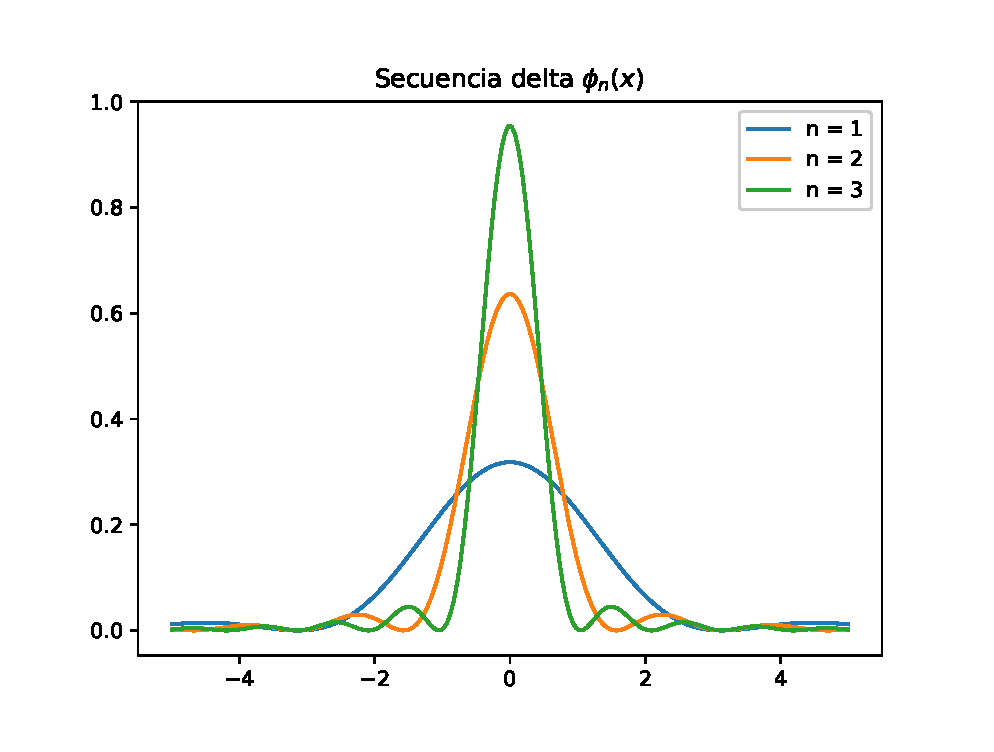
\includegraphics[scale=0.8]{Imagenes/secuencia_delta_03.eps}
%     \caption{Secuencia para $\phi_{n}$ con una función $\sin^{2}(x)/x$}
%     \label{fig:plot_secuencia_03}
% \end{figure}



% Tomemos en cuenta que no es correcto expresar que éstas secuencias convergen a la función delta: los límites de esas secuencias \emph{no existen} (de acuerdo a las definiciones conocidas de convergencia).

% Todas estas funciones están normalizadas a la unidad
% \begin{equation}
% \lim_{n \to \infty} \scaleint{6ex}_{\bs - \infty}^{+ \infty} \phi_{n}(x) \: \dd{x} = 1
% \label{eq:ecuacion_delta_05}
% \end{equation}

% \subsection{Propiedades de la delta de Dirac.}

% Una vez que hemos definido la delta de Dirac, nos gustaría saber ahora como operar con y en ella. ¿Es posible decir algo sobre su derivada? La respuesta a esta pregunta es afirmativa y las secuencias delta hechas de funciones diferenciables nos permiten responder a la pregunta de manera precisa.
% \par
% Por ejemplo, sea la secuencia delta
% \begin{align*}
% \phi_{n} &= \dfrac{n}{\sqrt{\pi}} e^{-n^{2} x^{2}}
% \end{align*}
% entonces, al diferenciar la secuencia
% \begin{align*}
% \dv{\phi_{n}(x)}{x} = - \dfrac{2 \: n^{3}}{\sqrt{\pi}} \: x \: \exp(-n^{2} \: x^{2})
% \end{align*}
% \begin{figure}[H]
%     \centering
%     \includegraphics[scale=0.8]{Imagenes/secuencia_delta_04.eps}
%     \caption{Derivada de la secuencia delta.}
%     \label{fig:fig_figura_delta_04}
% \end{figure}
% Consideremos ahora la integral
% \begin{align*}
% \scaleint{6ex}_{\bs -\infty}^{+\infty} \dv{\phi_{n}(x)}{x} \: f(x) \dd{x}
% \end{align*}
% donde $f(x)$ es diferenciable. Integrando por partes, se obtiene
% \begin{align*}
% \scaleint{6ex}_{\bs -\infty}^{+\infty} \dv{\phi_{n}(x)}{x} \: f(x) \dd{x} = \phi_{n} \: f(x) \eval_{-\infty}^{+\infty} - \scaleint{6ex}_{\bs -\infty}^{+\infty} \phi_{n} \: \dv{f(x)}{x} \dd{x}
% \end{align*}
% Suponemos que
% \begin{align*}
% \lim_{n \to \infty} \left( \dfrac{n}{\sqrt{\pi}} \right) \exp(-n^{2} \: x^{2}) \: f(x) = 0
% \end{align*}
% Esto normalmente es cierto, ya que estamos considerando funciones para las cuales la integral
% \begin{align*}
% \scaleint{6ex}_{\bs -\infty}^{+\infty} \phi_{n}(x) \: f(x) \dd{x} 
% \end{align*}
% converge.
% \par
% Entonces, haciendo que $n \to \infty$, tenemos
% \begin{align*}
% \lim_{n \to \infty} \scaleint{6ex}_{\bs -\infty}^{+\infty} \dv{\phi_{n}(x)}{x} \: f(x) \dd{x} = - \lim_{n \to \infty} \phi_{n}(x) \: f^{\prime} (x) \dd{x} =  -f^{\prime}(0)
% \end{align*}
% Vemos entonces que la secuencia $\phi^{\prime}(x)$ está relacionada con la propiedad de filtro.
% \begin{propiedad}

% La delta de Dirac satisface varias propiedades y conocerlas es de mucha utilidad cuando resolvemos problemas específicos en física. 
% \par

\section{Introduciendo más variables.}
\subsection{Ampliando el uso de la delta.}

Será muy común utilizar la delta de Dirac cuando tengamos más variables,  por lo que es conveniente representar la $\delta (x)$ en el correspondiente sistema.
\begin{align}
\delta (\va{\bm{r}} - \va{\bm{r_{0}}}) = \delta (x - x_{0}) \: \delta (y - y_{0}) \: \delta (z - z_{0})
\label{eq:ecuacion_A_03}
\end{align}
de manera que al integrar sobre todo el espacio tenemos:
\begin{align*}
\scaleint{6ex} \delta (\va{\bm{r}} - \va{\bm{r_{0}}}) \: \dd{x} \dd{y}  \dd{z} = 1
\end{align*}

\noindent
\textbf{Ejemplo con más variables:} La función delta permite especificar la densidad de carga debida a un conjunto de $N$ cargas puntuales de valores $q_{i}$ situadas en posiciones $\va{r_{i}}$ como:
\begin{align}
\rho (\va{r}) = \nsum_{i=1}^{N} q_{i} \: \delta(\va{r} - \va{r_{i}})
\label{eq:ecuacion_A_04}
\end{align}
Las propiedades de la función delta permiten obtener el potencial $\varphi(\va{r})$ evaluando la función dentro de la integral en los puntos $\va{r_{i}}$, es decir:
\begin{align}
\varphi(\va{r}) &= \scaleint{6ex} \dfrac{\rho(\va{r^{\prime}})}{\abs{\va{r} - \va{r^{\prime}}}} \: d^{3}r^{\prime} =  \nsum_{i=1}^{N} q_{i} \scaleint{6ex} \dfrac{\delta ( \va{r} - \va{r_{i}})}{\abs{\va{r} - \va{r^{\prime}}}} \: d^{3}r^{\prime} = \nsum_{i=1}^{N} \dfrac{q_{i}}{\abs{\va{r} - \va{r_{i}}}}
\label{eq:ecuacion_A_05}
\end{align}
Nótese que $\delta (x)$ tiene unidades de inverso de $x$ y $\delta (\va{r})$ tiene unidades de densidad numérica.
\par
La $\delta (x)$ toma una forma particular en coordenadas cilíndricas y esféricas, dadas por la condición de normalización:
\begin{enumerate}
\item Para coordenadas cilíndricas:
\begin{align*}
&\scaleint{6ex} \delta (\va{r} - \va{r}_{0}) \: R \: \dd{R} \: \dd{\varphi} \: \dd{z} \\[0.5em]
&\Rightarrow \delta (\va{r}) =  \dfrac{1}{R} \: \delta (R {-} R_{0}) \: \delta (\varphi {-} \varphi_{0}) \: \delta (z {-} z_{0})
\end{align*}
\item Para coordenadas esféricas:
\begin{align*}
&\scaleint{6ex} \delta (\va{r} - \va{r}_{0}) \: r^{2} \, \dd{r} \, \sin \theta \, \dd{\theta} \, \dd{\varphi} = 1 \\
&\Rightarrow \delta (\va{r}) = \dfrac{1}{r^{2}} \: \delta (r {-} r_{0}) \, \delta (\cos \theta {-} \cos \theta_{0}) \, \delta (\varphi {-} \varphi_{0})
\end{align*}
\end{enumerate}

% Algunas funciones generan en el límite la función delta:
% \begin{align*}
% \delta(x) = \begin{cases}
% \displaystyle
% \lim_{\varepsilon \to 0^{+}} \dfrac{1}{\pi} \, \dfrac{\varepsilon}{x^{2} + \varepsilon^{2}} & \mbox{Lorentz} \\[1em]
% \displaystyle
% \lim_{\sigma \to 0^{+}} \dfrac{1}{\sigma \, \sqrt{2 \, \pi}} \, \exp \left( - \dfrac{x^{2}}{2 \, \sigma^{2}} \right) & \mbox{Gaussiana} \\[1em]
% \displaystyle \lim_{\varepsilon \to 0^{+}} \dfrac{\sin(x / \varepsilon)}{ \pi \, x} & \mbox{Dirichlet} \\[1em]
% \displaystyle \lim_{L \to \infty} \dfrac{1}{2 \, \pi} \scaleint{6ex}_{\bs - \abs{L}}^{\abs{L}} \exp(i \, k \, x) \dd{k} & \mbox{Fourier}
% \end{cases}
% \end{align*}
% \section*{Ejercicios a cuenta}
% \begin{enumerate}[label=\roman*.]
% \item Demuestra que 
% \[ \nabla \vdot \left( \dfrac{e_{r}}{r^{2}} \right) = 0 \hspace{1cm} \mbox{para } r > 0 \]
% Tip: Se puede resolver en coordenadas cartesianas, pero es más fácil usando coordenadas esféricas.
% \item Demuestra que 
% \[ \nabla \left( \dfrac{1}{r} \right) = - \dfrac{e_{r}}{r^{2}} \]
% \end{enumerate}


\section{Ejemplos.}

\noindent
\textbf{Ejemplo 1} Evalúa la siguiente integral:
\begin{align*}
\scaleint{6ex}_{\bs -4}^{+7} (x^{3} - 3 \, x^{2} + 2 \, x + 1) \, \delta(x + 2) \dd{x}
\end{align*}

El único punto en el cual la integral no es igual a cero es en el punto $x = -2$, en donde la evaluación depende únicamente del valor que tenga la función $f(x = -2)$:
\begin{align*}
(-2)^{3} - 3 (-2)^{2} + 2(-2) + 1 = -23
\end{align*}

\noindent
\textbf{Ejemplo 2} Evalúa la siguiente integral:
\begin{align*}
\scaleint{6ex}_{\bs -2}^{+4} e^{2 \abs{x}-4} \, \delta(x + 5) \dd{x}
\end{align*}

En este caso la integral es igual a cero, puesto que el punto en el cual la delta de Dirac aplica su efectividad, $x = -5$, está fuera de los límites de la integración $-2$ y $+4$.

\rule{0.9\textwidth}{0.1mm} \\
Podemos aprovechar el resultado de la integración, ya que es tan buena que incluso se puede definir la derivada de la función delta de Dirac con respecto a $x_{0}$.
\begin{align*}
\scaleint{6ex}_{\bs -\infty}^{\infty} f(x) \, \ptilde{\delta} (x - x_{0}) \dd{x} = - \ptilde{f}(x_{0})
\end{align*}

Es posible obtener las derivadas de orden superior mediante la expresión:
\begin{align*}
\scaleint{6ex}_{\bs -\infty}^{\infty} &f(x) \, \delta^{(n)} (x - x_{0}) \dd{x} = \begin{cases}
(-1)^{n} \, \ntilde{f}{n} (x_{0}) & \mbox{si } a < x_{0} < b \\
0 & \mbox{de otra manera}
\end{cases}
\end{align*}   

La delta de Dirac satisface la siguiente relación:
\begin{align*}
\delta(g(x)) = \nsum_{k=1}^{n} \dfrac{\delta(x - c_{k})}{\abs{\ptilde{g}(c_{k})}}, \hspace{0.5cm} \ptilde{g}(c_{k}) \neq 0
\end{align*}
donde $\left\{ c_{k} \right\}_{k=1}^{n}$ son todas las raíces de la ecuación $g(x) = 0$.

\begin{align*}
\scaleint{6ex}_{\bs a}^{b} &f(x) \, \ptilde{\delta}(g(x)) \dd{x} = \begin{cases}
- \displaystyle \nsum_{k=1}^{n} \dfrac{\ptilde{f}(c_{k})}{\ptilde{g}(c_{k})} & \mbox{si } a < c_{k} < b \\
0 & \mbox{de otra manera}
\end{cases}
\end{align*}

\rule{0.9\textwidth}{0.1mm}

\noindent
\textbf{Ejemplo 3}. Evalúa la siguiente integral:
\begin{align*}
I \equiv \scaleint{6ex}_{\bs -\infty}^{\infty} f(t) \, \delta(t^{2} - a^{2}) \dd{t}
\end{align*}
donde $f(t)$ es una función suave y $a$ es una constante real.

Identificamos que $g(t)$ como $(t^{2} - a^{2})$,  que tiene raíces $c_{1} = -a$ y $c_{2} = a$, con la primera derivada $\ptilde{g}(t) = 2 \, t$, por lo que tendremos:
\begin{eqnarray*}
\delta(t^{2} - a^{2}) &=&  \dfrac{\delta (t - c_{1})}{\abs{\ptilde{g}(c_{1})}} + \dfrac{\delta (t - c_{2})}{\abs{\ptilde{g}(c_{2})}} = \\[0.5cm] 
&=& \dfrac{\delta (t - (-a))}{\abs{-2a}} + \dfrac{\delta (t - a)}{\abs{2a}} = \\[0.5em] 
&=& \dfrac{1}{2 \abs{a}} \big[ \delta(t + a) + \delta(t - a) \big]
\end{eqnarray*}
Sustituyendo en la integral obtenemos:
\begin{eqnarray*}
I &=& \dfrac{1}{2 \abs{a}} \scaleint{6ex}_{\bs -\infty}^{\infty} f(t) \, \big[ \delta(t {+} a) + \delta(t {-} a) \big] \dd{t} = \\[0.5em] 
&=& \dfrac{1}{2 \abs{a}} \left\{ \scaleint{6ex}_{\bs -\infty}^{\infty} f(t) \, \delta(t {+} a) \dd{t} {+} \scaleint{6ex}_{\bs -\infty}^{\infty} f(t) \, \delta(t {-} a) \dd{t} \right\} \\[0.5em] 
&=& \dfrac{1}{2 \abs{a}} \bigg[ f(-a) + f(a) \bigg]
\end{eqnarray*}
Vemos que la integral se anula (como es de esperarse) si la función $f$ es impar.

\noindent
\textbf{Ejemplo 4. } Evalúa la integral:
\begin{align*}
\scaleint{6ex}_{\bs 1}^{\infty} \sin t \, \delta \left( t^{2} - \dfrac{\pi}{4} \right) \dd{t}
\end{align*}

Vemos que:
\begin{align*}
g(t) = t^{2} - \dfrac{\pi}{4}, \hspace{1.5cm} c_{1} = \dfrac{\pi}{2}, \hspace{0.3cm} c_{2} = - \dfrac{\pi}{2}
\end{align*}

Usamos solo la raíz positiva en el rango de integración. Además: $\ptilde{g}(t) =  2 \, t$, entonces: 
\begin{align*}
\scaleint{6ex}_{\bs 1}^{\infty} \sin t \, \delta \left( t^{2} - \dfrac{\pi}{4} \right) \dd{t} =  \dfrac{f(c_{1})}{\abs{\ptilde{g}(c_{1})}} = \dfrac{\sin (\pi/2)}{\pi} = \dfrac{1}{\pi}
\end{align*}

En el otro caso:
\begin{align*}
\scaleint{6ex}_{\bs -\infty}^{\infty} \sin t \, \delta \left( t^{2} - \dfrac{\pi}{4} \right) \dd{t} = 0
\end{align*}
ya que con la segunda raíz $c_{2}$ que también está en el rango de integración, pero su contribución cancela la de $c_{1}$.

\noindent
\textbf{Ejemplo 5. } Evalúa la integral:
\begin{align*}
\scaleint{6ex}_{\bs 0}^{\infty} \ln z \, \delta (z^{2} - 4 ) \dd{z}
\end{align*}

Vemos que $g(z) = z^{2} - 4$, la cual tiene dos raíces $c_{1} = 2$ y $c_{2} = -2$, de las cuales solo la raíz positiva está en el rango de integración.

Entonces, con $\ptilde{g}(z) = 2 \, z$, tenemos:
\begin{eqnarray*}
\scaleint{6ex}_{\bs 0}^{\infty} \ln z \, \delta (z^{2} - 4 ) \dd{z} &=& \dfrac{f(c_{1})}{\abs{\ptilde{g}(c_{1})}} = \\[0.5em] 
&=& \dfrac{\ln (c_{1})}{\abs{2 c_{1}}} \\[0.5em] 
&=& \dfrac{\ln 2}{4} =  0.1733
\end{eqnarray*}
    
\end{document}